\documentclass[a4peper, 12pt, titlepage, finall]{report}

%различные пакеты

\usepackage[T1, T2A]{fontenc}
\usepackage[russian]{babel}
\usepackage[backend=bibtex]{biblatex}
\usepackage{tikz}
\usepackage{geometry}
\usepackage{indentfirst}
\usepackage{fontspec}
\usepackage{graphicx}
\usepackage{array}
\graphicspath{{./images/}}

\usetikzlibrary{positioning, arrows}

\geometry{a4paper, left = 15mm, top = 10mm, bottom = 20mm, right = 15mm}

\setmainfont{Spectral Light}%{Times New Roman}
\setmonofont{Courier New}
%\setcounter{secnumdepth}{3}
%\setcounter{tocdepth}{3}

\bibliography{overview} 

\begin{document}

    \begin{titlepage}
        \begin{center}
            {\small \sc Московский государственный университет имени М.~В.~Ломоносова\\
            Факультет вычислительной математики и кибирнетики\\
            Кафедра автоматизации систем вычислительных комплексов\\}
            \vfill
            {\large \sc Курсовая работа}\\~\\

            {\large \bf Анализ и исследование структур данных для поиска в таблицах классификации в архитектуре сетевого процессора без выделенного ассоциативного устройства}\\~\\

        \end{center}
        
        \begin{flushright}
            \vfill
            \vfill
            {Никифоров Никита Игоревич, 321 группа}\\
            {Научные руководители: Волканов Д. Ю., Скобцова Ю. А}
        \end{flushright}

        \begin{center}
            \vfill
            {\small Москва\\2019}
        \end{center}
    \end{titlepage}

    \chapter*{Аннтотация}
        В данной курсовой работе рассматривается проблема классификации пакетов в рамках архитектуры СПУ. В качестве критериев выбора структур данных были минимизация 
        используемой памяти и минимизация времени классификации. Был сделан обзор существующих структур данных, на его основе была выбрана {\ttfamily такая-то} 
        структура данных. Выбранная структура данных была реализована на эмуляторе архитектуры СПУ.
        
    \newpage
    \tableofcontents
    \newpage

    \chapter*{Введение}
        \addcontentsline{toc}{chapter}{\protect\numberline{}Введение}%
        В настоящее время ведётся активная разработка ПКС сетей, в которых требутся высокопроизводительных коммутаторов.
        Возникает задача разработки СПУ, являющегося основным элементом коммутаторов. СПУ - сетевое процессорное устройство
        представляет из себя интегральную микросхему, выполняющую следующие функции:
        \begin{enumerate}
            \item Получение пакетов с физического порта
            \item Выделение заголовка
            \item Классификация пакета по его заголовку
            \item Принятие решение о дальнейшем пути следования пакета
            \item Управление очередями
            \item Отправка пакета на физический порт
    
        \end{enumerate}
        Заголовок пакета представляет из себя битовую строку, содержащую в себе признаки пакета, которые также являются битовыми строками.
        Для классификации пакетов используются таблицы классификации -- набор правил содержащих в себе признаки и действия над пакетом.
        Определения соответствия пакета правилам производится по выделенным из заголовка признакам, данный процесс называется классификацией.
        Разрабатываются соответствующие архитектуры СПУ, в которых в основновном используется ассоциативное устройство памяти для 
        хранения таблиц классификации, его использование оправданно скоростью, с которой оно позволяет выполнять классификацию пакетов.
        Так же ведутся разработки архитектуры СПУ без использования ассоциативного устройства памяти.
        В данной работе рассматривалась архитектура без выделенного ассоциативного устройства. Существуют различные виды и реализации 
        структур данных для выполнения классификации пакетов\cite{chao2007high:1}, 
        но так как в работе рассматривается конкретная архитектура, невозможно применить существующие реализации напрямую. 
        Поэтому в данной работе стояла задача разработать структуру данных
        непосредственно для данной архитектуры СПУ. Для выполнения этой задачи был проведён обзор структур данных и....       
    

    \chapter{Цели и задачи работы}
        Целью данной работы является исследование и разработка структур данных и алгоритм для поиска в
        рамках архитектуры СПУ без выделенного ассоциативного устройства.
        Для достижения поставленной цели необходимо было выполнить следующие задачи:
        \begin{enumerate}
            \item Провести обзор структур данных для оптимальному поиску в таблицах классификации пакетов с целью выбора для применения в рассматриваемой архитектуре процессора.
            \item Реализовать выбранные структуры данных и алгоритмы поиска в эмуляторе сетевого процессора.
            \item Провести экспериментальное исследование реализованных структур данных.
        \end{enumerate}
       
    \chapter{Рассматриваяемая архитектура СПУ}
        Из особенностей рассматриваемой архитектуры можно выделеть отсутствие ассоциативного устройства памяти и конвейерную архитектуру. 
        Они непосредственно влияют на ограничения предъявляемые к реализуемой структуре данных. В СПУ используется конвейерная 
        архитектура, каждый конвейер состоит из 10 вычислительных блоков. Вычислительный блок - это набор более низкоуровневых устройств,
        которые в данной работе не рассматриваются. Каждый вычеслительный блок имеет доступ к участку памяти в котором располагаются микрокод и данные.
        Из-за особенностей микроархитектуры, отсутствует отдельная область памяти, в которой хранятся данные. Поэтому микрокод содержит в себе все данные,
        необходимые для классификации пакетов.
        \begin{figure}[h]
            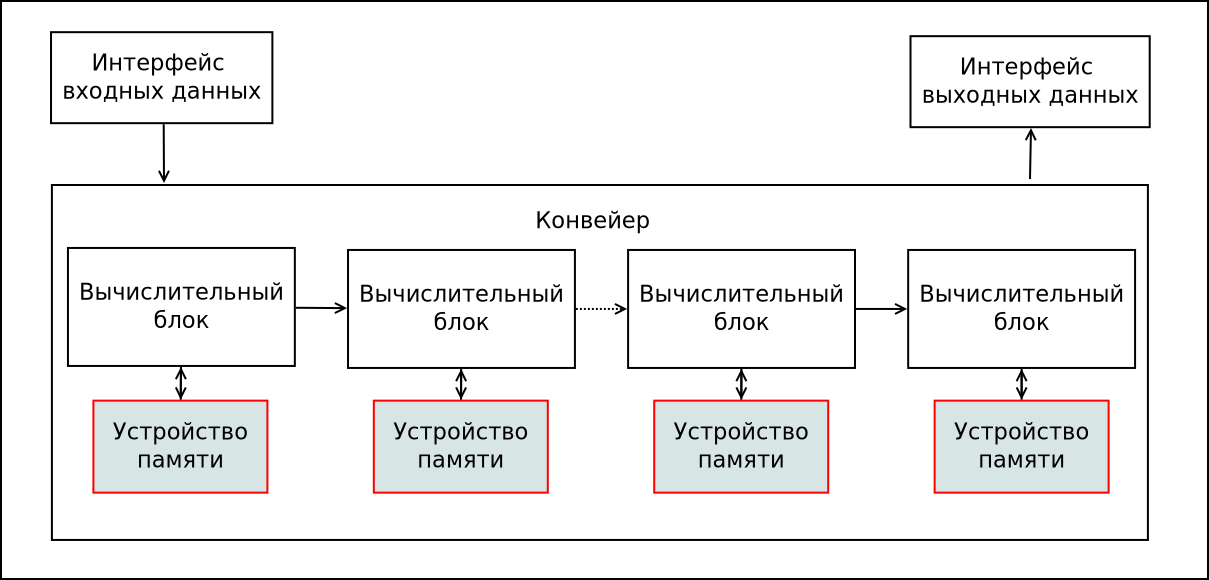
\includegraphics[width=\textwidth]{npu_all.png}
            \caption{Архитектура рассматриваемого СПУ}
        \end{figure}
        Для достяжения требуемой производительности в архитектуре используется ограничение на количество тактов обработки пакета
        на одном вычислительном блоке. Каждый пакет может обрабатываться на одном вычислительном блоке не более чем 25 тактов.
        
    \chapter{Постановка задачи} 
        Разработать структуру данных для классификации пакетов в рамках рассматриваемой архитектуры СПУ без выделенного ассоциативного устройства. 
        Из-за ограничений связанных с рассматриваемой архитектурой СПУ к реализуемой структуре данных предъявляются следующие требования:
        \begin{itemize}
            \item Объём памяти занимаемый структурой данной данных не должен превышать 2 мегабайт, это обусловлено ограничением количества памяти внутри одного вычислительного блока
            \item Количество тактов затраченных на поиск не должно превышать 250 тактов, данное требование обусловлено ограничением на количество тактов исполняемой программы внутри
                вычислительного блока.
            \item Реализуемая структура данных должна быть универсальна.
        \end{itemize}
    \chapter{Обзор структур данных для классификация пакетов в рамках рассматриваемой архитектуре СПУ}
            Целью данного обзора является сравнение и выбор структур данных для поиска в таблицах классификации. 
            Для достижения поставленной цели, необходимо было выполнить следующие задачи:

            В силу особенностей архитектуры СПУ, а именно отсутствие адресуемой памяти, 
            которая требуется для не древовидных структур данных будут рассматриваться только древовидные структуры данных. 
            Под памятью занимаемой структурой данных понимается  {\ttfamily   N * 128 = memmory} , где {\ttfamily N} - количество 
            инструкций в конкретной реализации рассматриваемой структуры данных, 128 - бит на одну инструкцию.
    
        В настоящем обзоре использовались следующие критерии:
        \begin{enumerate}
            \item Асимтотическая сложность поиска - позволяет оценить использование ресурсов СПУ, для поиска в структуре данных.
            \item Универсальность структуры данных - используемая структура данных должна поддерживать поиск произвольных битовых строк
                  не превосходящих по длине 128 бит.
            \item Дополнительные данные необходимые для построения структуры данных.
            \item Необходимость использования адресуемой памяти - некоторым рассматриваемым структурам данных требуется адресуемая память для их реализации, соответствующей их асимптотической сложности.
            \item Количество вершин, которое необходимо посетить для поиска в худшем случае.
            \item Возможность оптимизации алгоритма поиска с помощью инструкций микроархитектуры ядерконвейера СПУ.
            \item Необходимость изменения микроархитектуры ядер конвейера СПУ.
            \item Оценка памяти занимаемой структурой данных - рассматривается структура данных для 10000 вождений префиксов IPv4.
            \item Сложность добавления и удаления элементов из рассматриваемой структуры данных.
        \end{enumerate}

        Сравнение структур данных будет провоодиться по критериям 1, 2, 4, 5, 8.

    \section{Структуры данных для классификации пакетов в рамках рассматриваемой архитектуры СПУ}
        \subsection{Двоичное однобитное дерево}
            Наиболее распространенная структура данных для LPM. Строится дерево по заданным префиксам, 
            так что каждому биту префикса соответствует своя вершина в дереве. 
            Поиск осуществляется спуском в глубину по битам элемента, для которого выполняется поиск. 
            Поиск заканчивается тогда, когда достигнута пустая вершина, результатом поиска считается последний встретившийся префикс. 
            На Рис. 1 изображён пример данного дерева для набора префиксов.

            \begin{figure}[h]      
                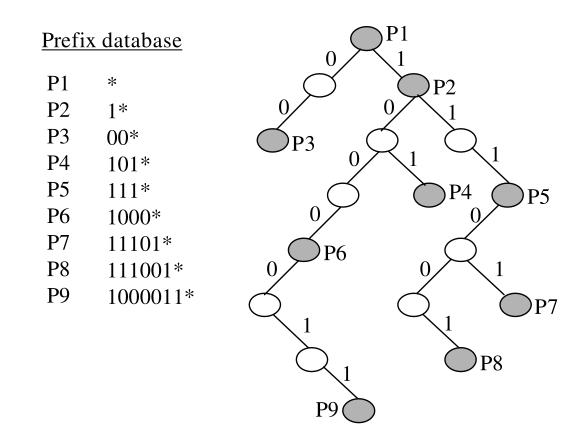
\includegraphics[width=\textwidth]{one_bit_tree.png}
                \caption{Пример построения двоичного однобитного дерева}
                \label{fig:mesh1}
            \end{figure}

            \underline{Асимптотическая сложность поиска} для этой структуры данных соответствует {\ttfamily $O(W)$},\\
            где {\ttfamily W} - максимальная длина префикса.\\
            \underline{Универсальность структуры данных} - рассматриваемое дерево может быть использовано для любых данных представимых в битовом виде.\\
            \underline{Дополнительные данные для построения} структуры данных не требуются.\\
            \underline{Количество вершин которое необходимо посетить для поиска} не превосходит 128.
            {\ttfamily (Коментарий: тут вообще имеется в виду худший случай, т.е. кода мы ищем префикс IPv6\\ длиной 128 бит. При этом он есть в дереве и есть все префиксы до него.)}\\
            \underline{Оптимизацию агоритма поиска} проводить не требуется.\\
            \underline{Изменение микроархитектуры ядер конвейера СПУ} не требуется для реализации данного алгоритма.\\
            \underline{Оценка памяти занимаемой структурой данных} - Будем считать, что на каждую вершину используется не более 5 инструкций,
            тогда рассматриваемая структура данных занимает не более чем 15000 Кбайт.\\
            \underline{Добавление и удаление элементов} из рассматриваемой структуры данных имеет асимптотическую сложность 
            {\ttfamily $O(\log_2{W})$}, где {\ttfamily W} - максимальная длина префикса и не требует перестройки всей структуры данных.\\

        \subsection{Сжатое двоичное дерево}
            Рассматриваемая структура данных -- пришедшая со временем оптимизация двоичного однобитного дерево. Сначала строится двоичное однобитное дерево.
            далее оно сжимается, то есть все вершины у которых только один лист сокращаются, и в следующую вершину заносятся данные о 
            количестве пропущенных вершин. Таким образом построенное дерево не имеет вершин с одним листом. Благодаря описанной оптимизации данное дерево
            занимает гораздо меньше памяти. Это обусловлено отсутствием проходных вершин. Однако, уменьшает количество затраченных инструкций на поиск лишь 
            для префиксов, перед которыми были однолистные вершины. Для худшего случая, когда для префикса есть все его более короткие версии, количество вершин, 
            которые нужно посетить для поиска анологично двоичному однобитному дереву.

            \begin{figure}[h]
                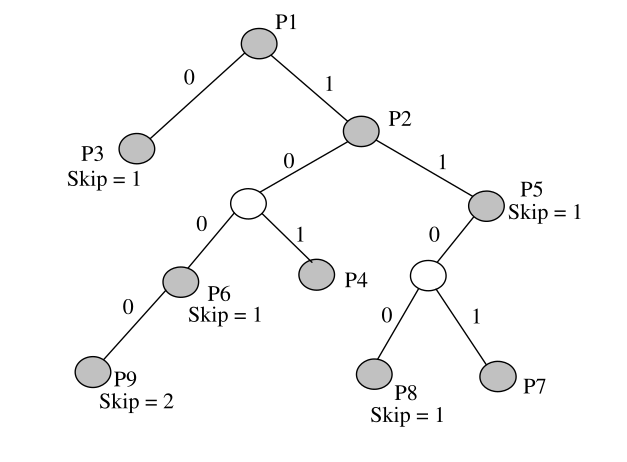
\includegraphics[width=\textwidth]{patricia_trie.png}
                \caption{Пример построения сжатого двоичного дерева}
                \label{fig:mesh2}
            \end{figure}

            \underline{Асимптотическая сложность поиска} для этой структуры данных соответствует {\ttfamily $O(W)$},\\
            где {\ttfamily W} - максимальная длина префикса.\\
            \underline{Универсальность структуры данных} - рассматриваемое дерево может быть использовано для любых данных представимых в битовом виде.\\
            \underline{Дополнительные данные} для построения структуры данных не требуются.\\
            \underline{Количество вершин которое необходимо посетить для поиска} не превосходит 128.\\
            \underline{Оптимизацию агоритма поиска} проводить не требуется.\\
            \underline{Изменение микроархитектуры ядер конвейера СПУ} не требуется для реализации данного алгоритма.\\
            \underline{Оценка памяти занимаемой структурой данных} - рассматриваемая структура данных занимает не более чем 8000Кбайт.\\
            \underline{Добавление и удаление элементов} из рассматриваемой структуры данных имеет асимптотическую сложность 
            {\ttfamily $O(\log_2{W})$}, где {\ttfamily W} - максимальная длина префикса и не требует перестройки всей структуры данных.\\
        
        \subsection{Мультибитное сжатое дерево}
            Данное дерево -- оптимизация двоичного сжатого дерева. Используется другая стуктура деревьев, когда в каждой вершине
            может быть максимум не два листа, а {\ttfamily $2^h$}, где {\ttfamily h} -- это максимальная глубина поддерева данной вершины.
            При использовании рассматриваемой структуры данных в рамках архитектуры процессора общего назначение, количество операций для поиска ограничевается глубиной дерева,
            которая равна {\ttfamily $\frac{W}{K}$}, где {\ttfamily W} -- длина максимального префикса, а {\ttfamily K} -- количество уровней в нашем дереве.
            В рамках архитектуры СПУ будет рассматриваться реализация данного дерева, в которой используется линейный поиск в каждой вершине по дочерним вершинам.

            \begin{figure}[h]
                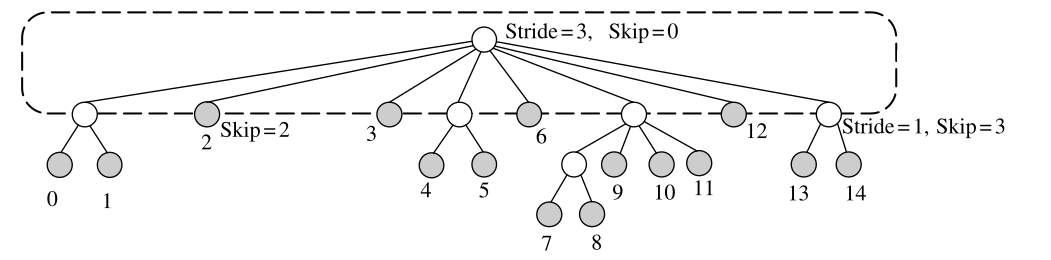
\includegraphics[width=\textwidth]{level_compressed_trie.png}
                \caption{Пример построения мультибитного сжатого дерева}
                \label{fig:mesh3}
            \end{figure}

            \underline{Асимптотическая сложность поиска} для этой структуры данных соответствует {\ttfamily $O(\frac{W}{K}*N)$},\\
            где {\ttfamily K} - количество префиксов в рассматриваемой структуре данных, а {\ttfamily W} - максимальная длина префикса
            и {\ttfamily N} -- количество листьев в вершине.\\
            \underline{Универсальность структуры данных} - рассматриваемое дерево может быть использовано для любых данных представимых в битовом виде.\\
            \underline{Дополнительные данные} для построения структуры данных не требуются.\\
            \underline{Количество вершин которое необходимо посетить для поиска} не превосходит 30. 
            {\ttfamily Коментарий: Тут надо как-то сказать, что вершин то мы посещяем мало, а вот инструкций на каждую вершину много}\\
            \underline{Оптимизацию агоритма поиска} нужна, для организации бастрого доступа к листьям внутри одной вершины.\\ 
            \underline{Изменение микроархитектуры ядер конвейера СПУ} для данной реализации не требуется.\\
            \underline{Оценка памяти занимаемой структурой данных} - Будем считать, что каждая вершина занимает 15 инструкций в среднем, из-за линейного поиска по листьям. 
            Тогда рассматриваемая структура данных занимает не более чем 18000 Кбайт.\\
            \underline{Добавление и удаление элементов} из рассматриваемой структуры данных имеет асимптотическую сложность 
            {\ttfamily $O(\log_2{W})$}, где {\ttfamily W} - максимальная длина префикса и не требует перестройки всей структуры данных.\\
            
            При реализации микроинструкции, которая по заданной метке перехода и маске переходит на инструкцию находящуюся на метке + значение регистра с применённой маской,
            есть возможность реализовать структуру данных, в которой алгоритм поиска будет быстрее. Рассмотрим эту структуру данных в рамках архитектурвы с добавлением указанной микроинструкции.\\

            \underline{Асимптотическая сложность поиска} для этой структуры данных соответствует {\ttfamily $O(\frac{W}{K})$},\\
            где {\ttfamily K} - количество префиксов в рассматриваемой структуре данных, а {\ttfamily W} - максимальная длина префикса.
            \underline{Универсальность структуры данных} - рассматриваемое дерево может быть использовано для любых данных представимых в битовом виде.\\
            \underline{Дополнительные данные} для построения структуры данных не требуются.\\
            \underline{Количество вершин которое необходимо посетить для поиска} не превосходит 30.\\
            \underline{Оптимизацию агоритма поиска} нужна, для организации бастрого доступа к листьям внутри одной вершины.\\ 
            \underline{Изменение микроархитектуры ядер конвейера СПУ} требуется аппаратная реализации быстрого перехода внутри одной вершины.
            А именно необходима инструкция, которая по заданной метке перехода и маске переходит на инструкцию находящуюся на метке + значение регистра с применённой маской.\\
            \underline{Оценка памяти занимаемой структурой данных} - Будем считать, что каждая вершина занимает 5 инструкций, благодаря новой микроинструкции.
            Тогда рассматриваемая структура данных занимает не более чем 7000 Кбайт.\\
            \underline{Добавление и удаление элементов} из рассматриваемой структуры данных имеет асимптотическую сложность 
            {\ttfamily $O(\log_2{W})$}, где {\ttfamily W} - максимальная длина префикса и не требует перестройки всей структуры данных.\\
            

        \subsection{Бинарный поиск по длинам префиксов}
            Структура данных основана на построении специальных таблиц для префиксов определённой длины. Пусть максимальная длина префикса {\ttfamily W}, 
            тогда строятся таблицы {\ttfamily $h_{1}...h_{w}$}. В каждой из них хранятся префиксы длины соответствующие номеру этой таблицы. Предполагается, 
            что в каждой такой таблице реализована своя хеш-функция, которая быстро позволяет найти вхождение префикса в данную таблицу.
            Таким образом мы можем выполнить бинарный поиск по длине префиксов. В рамках рассматриваемой архитектуры СПУ, реализация таких таблиц возможна только
            с использованием древовидных структур данных.

            \begin{figure}[h]
                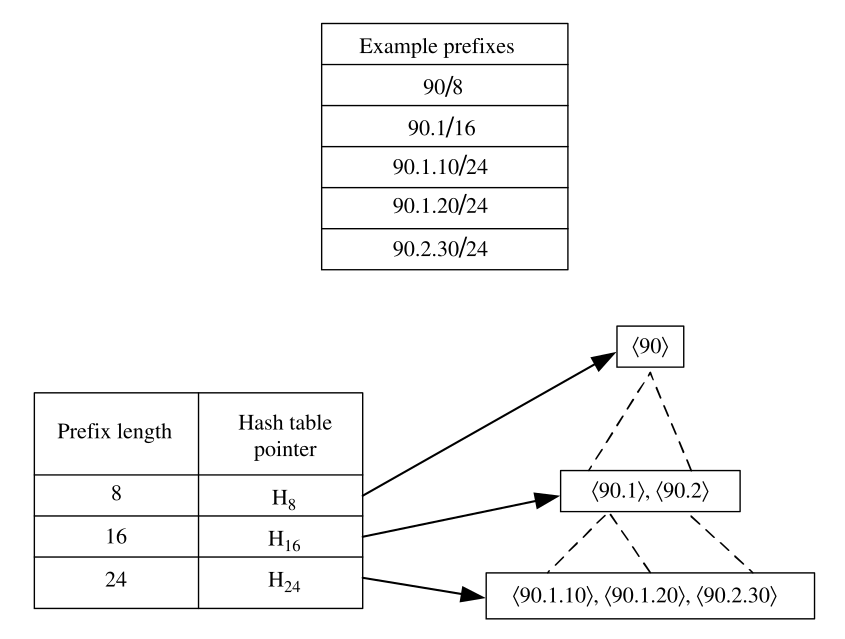
\includegraphics[width=\textwidth]{binary_search.png}
                \caption{Пример бинарного поиска по длинам префиксов}
                \label{fig:mesh4}
            \end{figure}


            \underline{Асимптотическая сложность поиска для этой структуры данных} соответствует {\ttfamily $O(K*\log_2{N})$},\\
            где {\ttfamily K} - количество префиксов в рассматриваемой структуре данных, а {\ttfamily W} - максимальная длина префикса.
            и {\ttfamily N} -- количество префиксов в таблице.\\
            \underline{Универсальность структуры данных} - рассматриваемая структура данных может быть использовано только для поиска префиксов.\\
            \underline{Дополнительные данные} для построения структуры данных не требуются.\\
            \underline{Количество вершин которое необходимо посетить для поиска} не превосходит 128.\\
            \underline{Оптимизацию агоритма поиска} требуется, а именно необходима для реализации поиска внутри таблицы.\\
            \underline{Изменение микроархитектуры ядер конвейера СПУ} требуется аппаратная реализация хеш-функций.\\
            \underline{Оценка памяти занимаемой структурой данных} - рассматриваемая структура данных занимает не более чем {\ttfamily TODO: рассчитать} Кбайт.\\
            \underline{Добавление и удаление элементов} из рассматриваемой структуры данных требует перестройки всей структуры данных.\\


        \subsection{АВЛ дерево}
            Представление префиксов как скалярных префиксов позволяет использовать больший набор структур данных. 
            В качестве примера рассмотрим AVL дерево, основной особенностью которого является правило его построения: у каждой вершины разность 
            глубины левого и правого поддерева не превосходит 1, что даёт ассимптотическую сложность поиска {\ttfamily $O(1+\log_2{N})$}, 
            где {\ttfamily N} -- количество префиксов в нашей структуре данных. Из этого следует, что время поиска не зависит от длины искомых данных,
            а значит с помощью данной структуры данных очень эффективно выполнять поиск префиксов IPv6.
            \\
            \begin{figure}[h]
                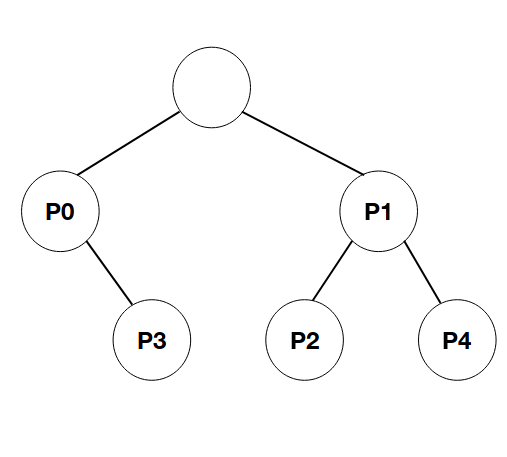
\includegraphics[width=\textwidth]{AVL-tree.png}
                \caption{Пример построения АВЛ дерева}
                \label{fig:mesh5}
            \end{figure}
            \\
            \\
            \underline{Асимптотическая сложность поиска для этой структуры данных} соответствует {\ttfamily $O(1 + \log_2{N})$},
            где {\ttfamily N} -- количество префиксов в таблице.\\
            \underline{Универсальность структуры данных} - рассматриваемое дерево может быть использовано для любых данных представимых в битовом виде.\\
            \underline{Дополнительные данные для построения структуры данных} не требуются.\\
            \underline{Количество вершин которое необходимо посетить для поиска} не превосходит 20.\\
            \underline{Оптимизацию агоритма поиска} проводить не требуется.\\
            \underline{Изменение микроархитектуры ядер конвейера СПУ} не требуется.\\
            \underline{Оценка памяти занимаемой структурой данных} - рассматриваемая структура данных занимает не более чем {\ttfamily TODO: рассчитать} Кбайт.\\
            \underline{Добавление и удаление элементов из рассматриваемой структуры данных} имеет логарифмическую сложность, и не требует перестройки всей структуры данных.\\


    \section{Сравнение структур данных}
        Для сравнения структур данных рассмотрим Таблицу 2.1 сравнения по критериям: ассимптотическая сложность, универсальность структуры данных,
        количество вершин, которое необходимо поситить для поиска и оценка памяти занимаемой структурой данных. 
        \begin{table}[ht]
            \begin{tabular}{|m{3cm} | m{2.5cm} | m{3.5cm} | m{4cm} | m{3.2cm}|}
                \hline
                \multicolumn{5}{|c|}{Сравнение структур данных}\\
                \hline
                \bf Название структуры данных     & \bf Сложность поиска & \bf Универсальность & \bf Количество вершин необходимых для поиска & \bf Память, Кбайт \\
                \hline
                Двоичное однобитное дерево & $O(W)$ & да & 128 & 15000 \\
                \hline
                Двоичное сжатое дерево & $O(W)$ & да & 128 & 8000 \\
                \hline
                Мультибитно сжатое дерево & $O(\frac{W}{K}*L)$ & да & 32 & 18000 \\
                \hline
                Бинарный поиск по длинам префиксов & $O(K*\log_2{N})$ & нет & 128 & {\ttfamily TODO} \\
                \hline
                АВЛ дерево & $O(1 + \log_2{N})$ & да & 20 & {\ttfamily TODO} \\
                \hline
            \end{tabular}
            \caption{Сравнение структур данных}
            {\ttfamily W - максимальная длина префикса, N - количество префиксов в структуре данных, L - количество дочерних вершин, К - глубина дерева, T - количество таблиц}
        \end{table}
        У каждой рассмотренной структуры данных есть свои достоинства и недостатки, рассмотрим их:
        \begin{enumerate}
            \item \underline{Binary one bit tree} данная структура проста в реализации, но занимает много памяти и поиск требует прохождения 128 вершин.
            \item \underline{Path Compressed trie} занимает меньше памяти, чем Binary one bit tree, но поиск требует прохождения 128 вершин. 
                Соответственно использование данного дерева предпочтительнее, чем Binary one bit tree.
            \item \underline{Level Compressed trie} занимает много памяти, но поиск требует прохождения сильно меньшего количества вершин. 
                Из-за проблем с реализацией в рамках рассматриваемой архитектуры, эта структура данных не может быть реализованна.
            \item \underline{Binary search on prefix length} занимает много памяти, и может быть использовано только для LPM. 
                Также из-за проблем с реализацией на рассматриваемой архитектуре, данная структура не подходит для решения проблемы.
            \item \underline{AVL tree} занимает столько же памяти, как и Path Compressed trie, но при этом, поиск требует прохождения малого количества вершин,
                которое зависит от количества вхождений в структуру данных, а не от конкретного префикса.
        \end{enumerate}

    \section {Выводы}
        {\ttfamily TODO: написать выводы, сделаю это позже, потому что пока не могу полностью оценить рассматриваемые структуры данных.}


        \printbibliography

\end{document} 
